\section{\scshape Model}

\subsection{Opis modelu}
\begin{frame}{Opis modelu}
	\begin{itemize}
	\item Dane o propagacji dymu generowane przez FDS.
	\item Symulacja dyskretna.
	\item Automat komórkowy wykorzystujący sąsiedztwo. Moore'a
	\begin{center}	
	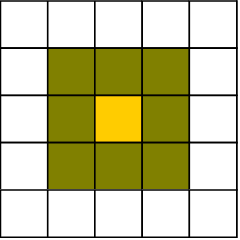
\includegraphics[keepaspectratio=true, scale=0.5]{moore}
	\end{center}
	\item Dynamiczne i statyczne pola potencjału.
	\item Wykorzystanie proksemiki.
	\end{itemize}
\end{frame}

\subsection{Teoria proksemiki}
\begin{frame}{Teoria proksemiki}
 \begin{itemize}
 	\item Reprezentacja pieszego przez elipsę.
 	\item Cztery możliwe orientacje.
 	\item Maksymalna powierzchnia intersekcji.
 	\begin{center}	
	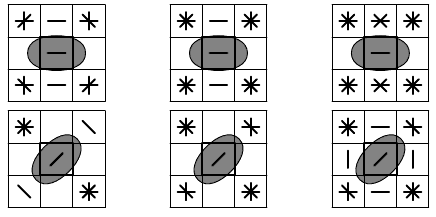
\includegraphics[keepaspectratio=true, scale = 0.5]{proxemics}
	\end{center}	
 \end{itemize}
\end{frame}

\subsection{Reprezentacja ewakuowanego}
\begin{frame}{Reprezentacja ewakuowanego}
\begin{itemize}
	\item Charakterystyka fizjologiczna.
	\item Trzy możliwe sposoby poruszania się.
	\item Wrażliwość na zmiany otoczenia.
	\item Czas reakcji.
\end{itemize}
\end{frame}

\subsection{Czas reakcji}
\begin{frame}{Czas reakcji}
\begin{center}	
	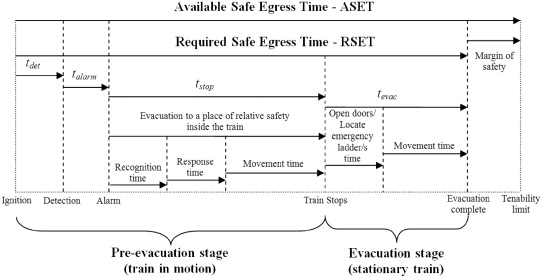
\includegraphics[scale=0.9]{egress_time}
\end{center}
\end{frame}

\subsection{Funkcja kosztu}
\begin{frame}{Funkcja kosztu}
\begin{center}
$q(F_{i,j}) = \alpha * S_{i,j} + \beta * D_{i,j}$
\end{center}

\begin{center}
$D{i,j} = dist + \gamma * \xi$
\end{center}

\begin{center}
$\xi = \alpha \cdot B^T$
\end{center}
\end{frame}